\chapter{异常}

\section{异常}

\subsection{异常(Exception)}

异常就是程序在运行过程中出现的非正常的情况,它可以被捕获并处理,以防止程序崩溃。\\

Exception是一个异常类,发生异常的时候会抛出一个异常对象。如果不处理异常,程序就会被中断。\\

\begin{table}[H]
    \centering
    \setlength{\tabcolsep}{5mm}{
        \begin{tabular}{|l|l|}
            \hline
            \textbf{异常}                  & \textbf{描述}              \\
            \hline
            ArithmeticException            & 异常的运算条件             \\
            \hline
            ArrayIndexOutOfBoundsException & 非法索引访问数组           \\
            \hline
            ClassCastException             & 不匹配的类型转换           \\
            \hline
            ClassNotFoundException         & 找不到相应类               \\
            \hline
            FileNotFoundException          & 文件无法找到               \\
            \hline
            IllegalArgumentException       & 非法参数                   \\
            \hline
            IndexOutOfBoundsException      & 索引超出范围               \\
            \hline
            InputMismatchException         & 输入类型不匹配             \\
            \hline
            NullPointerException           & 空指针异常                 \\
            \hline
            NumberFormatException          & 无法将字符串转换为数值类型 \\
            \hline
        \end{tabular}
    }
    \caption{常用异常}
\end{table}

例如当数组访问越界时,会抛出一个ArrayIndexOutOfBoundsException异常;当访问一个不存在的对象时,会抛出一个NullPointerException异常。\\

\subsection{捕获异常}

try-catch-finally结构可以用于捕获并处理异常,将可能出现异常的代码放在try结构中,将异常处理的代码放在catch结构中,finally结构中的代码无论是否出现异常都会执行。\\

当在try结构中出现异常时,程序会跳转到catch结构中,执行catch结构中的代码。一个异常被处理后,将不再影响程序的执行。\\

\begin{figure}[H]
    \centering
    
\includegraphics{img/Chapter7/7-1/1.png}
\end{figure}

\mybox{整除}

\begin{lstlisting}[language=Java]
import java.util.InputMismatchException;
import java.util.Scanner;

public class Division {
    public static void main(String[] args) {
        Scanner scanner = new Scanner(System.in);

        while (true) {
            try {
                System.out.print("Enter an integer for dividend: ");
                int dividend = scanner.nextInt();
                System.out.print("Enter an integer for divisor: ");
                int divisor = scanner.nextInt();
                int quotient = dividend / divisor;
                System.out.println(
                        dividend + " / " + divisor + " = " + quotient
                );
            } catch (InputMismatchException e) {
                System.out.println("Only integers supported.");
            } catch (ArithmeticException e) {
                System.out.println("Divisor cannot be 0.");
            } finally {
                scanner.nextLine();
            }
        }
    }
}
\end{lstlisting}

\begin{tcolorbox}
    \mybox{运行结果}
    \begin{verbatim}
Enter an integer for dividend: 21
Enter an integer for divisor: 4
21 / 4 = 5
Enter an integer for dividend: 5
Enter an integer for divisor: 0
Divisor cannot be 0.
Enter an integer for dividend: 3.6
Only integers supported.
	\end{verbatim}
\end{tcolorbox}

\vspace{0.5cm}

\subsection{throw}

throw关键字用于在方法内部抛出一个异常,throws关键字用于方法签名中,表示该方法可能会抛出异常。\\

抛出异常后,需要由方法的调用者来处理异常。如果调用者没有处理异常,那么异常就继续向上抛出,直到被处理。\\

\begin{figure}[H]
    \centering
    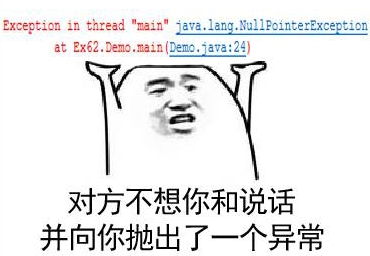
\includegraphics{img/Chapter7/7-1/2.png}
\end{figure}

\mybox{阶乘}

\begin{lstlisting}[language=Java]
import java.util.Scanner;

public class Factorial {
    public static void main(String[] args) {
        Scanner scanner = new Scanner(System.in);

        System.out.print("Enter n: ");
        int n = scanner.nextInt();

        try {
            System.out.println(n + "! = " + factorial(n));
        } catch (IllegalArgumentException e) {
            e.printStackTrace();
        } finally {
            scanner.close();
        }
    }

    public static int factorial(int n)
            throws IllegalArgumentException {
        if (n < 0) {
            throw new IllegalArgumentException(
                    "Factorial of negative numbers is not defined."
            );
        }

        if (n == 0 || n == 1) {
            return 1;
        }
        return n * factorial(n - 1);
    }
}
\end{lstlisting}

\begin{tcolorbox}
    \mybox{运行结果}
    \begin{verbatim}
Enter n: -1
java.lang.IllegalArgumentException: Factorial of negative 
numbers is not defined.
    at Factorial.factorial(Factorial.java:21)
    at Factorial.main(Factorial.java:11)
	\end{verbatim}
\end{tcolorbox}

\newpage

\section{自定义异常}

\subsection{自定义异常}

为了满足某些特定的需求,用户可以自定义异常,自定义异常继承于Exception类或其子类。自定义异常的目的是为了提供更具体和有意义的错误处理。\\

\mybox{库存}

\begin{lstlisting}[language=Java]
public class OutOfStockException extends Exception {
    public OutOfStockException(String msg) {
        super(msg);
    }
} 
\end{lstlisting}

\begin{lstlisting}[language=Java]
public class Product {
    private String name;
    private int stock;

    public Product(String name, int stock) {
        this.name = name;
        this.stock = stock;
    }

    public void purchase() throws OutOfStockException {
        if (stock <= 0) {
            throw new OutOfStockException(name + " is out of stock.");
        }
        stock--;
    }
}
\end{lstlisting}

\begin{lstlisting}[language=Java]
public class Purchase {
    public static void main(String[] args) {
        Product product = new Product("Cheeseburger", 50);

        try {
            for (int i = 0; i < 60; i++) {
                product.purchase();
            }
        } catch (OutOfStockException e) {
            e.printStackTrace();
        }
    }
}
\end{lstlisting}

\begin{tcolorbox}
    \mybox{运行结果}
    \begin{verbatim}
OutOfStockException: Cheeseburger is out of stock.
    at Product.purchase(Product.java:12)
    at Purchase.main(Purchase.java:7)
	\end{verbatim}
\end{tcolorbox}

\newpage